\documentclass[11pt,a4paper]{article}
\usepackage[paperwidth=13.333in,paperheight=7.5in,margin=0pt]{geometry}

\usepackage[utf8]{inputenc}
\usepackage[T1]{fontenc}
\usepackage{lmodern}
\usepackage{amsmath,amssymb,amsfonts,bm}
\usepackage{graphicx}
\graphicspath{{../img/}{./img/}{img/}}
\usepackage{xcolor}
\usepackage{tikz}
\usetikzlibrary{calc,shapes.geometric,positioning}
\usepackage{booktabs}
\usepackage{hyperref}

% Color Palette
\definecolor{navy}{HTML}{002060}
\definecolor{primaryblue}{HTML}{184C78}
\definecolor{accent}{HTML}{2980B9}
\definecolor{darkgray}{HTML}{2C3E50}
\definecolor{lightbg}{HTML}{F5F7FA}
\definecolor{bordergray}{HTML}{C8CDD2}
\definecolor{mutedgray}{HTML}{7F8C8D}
\definecolor{crimson}{HTML}{9E1636}
\definecolor{gold}{HTML}{B48C14}
\definecolor{successgreen}{HTML}{27AE60}

\pagestyle{empty}
\setlength{\parindent}{0pt}

% Total Slides Count
\newcommand{\totalslides}{27}

% Positioning helper
\newcommand{\at}[4]{%
  \node[anchor=north west,inner sep=0pt,text width=#3in,align=left]
    at ([xshift=#1in,yshift=-#2in]current page.north west) {#4\par};}

\newcommand{\fs}[2]{\fontsize{#1pt}{#2pt}\selectfont}

% Slide Header Macro
\newcommand{\slideheader}[3]{%
  % KU Logo
  \node[anchor=north west,inner sep=0pt]
    at ([xshift=0.5in,yshift=-0.2in]current page.north west)
    {
\includegraphics[width=0.9in]{ku_logo.png}};
  % Vertical accent bar
  \fill[accent] ([xshift=1.5in,yshift=-0.22in]current page.north west)
    rectangle ++(0.06in,-0.95in);
  % Category Tag and Title
  \at{1.68}{0.18}{11.1}{%
    {\fs{11.5}{14}\bfseries\color{accent}\MakeUppercase{#1}\quad|\quad}%
    {\fs{22}{26}\bfseries\color{navy}#2}\\[0.22em]
    \if\relax\detokenize{#3}\relax\else{\fs{13.5}{17}\color{darkgray}#3}\fi
  }
}

% Slide Footer Macro
\newcommand{\slidefooter}[1]{%
  % Dividing Line
  \fill[bordergray] ([xshift=0.5in,yshift=-7.0in]current page.north west)
    rectangle ++(12.333in,-0.02in);
  % Left Date
  \at{0.5}{7.06}{2.5}{\fs{10}{12}\color{mutedgray}November 3, 2026}
  % Center Presenter Info
  \node[anchor=north,inner sep=0pt]
    at ([yshift=-7.06in]current page.north)
    {\fs{10}{12}\color{mutedgray}Chong Shik Park, Ph.D. \enspace$|$\enspace Korea University, Sejong \enspace$|$\enspace AI Applications in Accelerators};
  % Right Slide Number
  \node[anchor=north east,inner sep=0pt]
    at ([xshift=-0.5in,yshift=-7.06in]current page.north east)
    {\fs{10}{12}\bfseries\color{primaryblue}#1 / \totalslides};
}

% Standard Full-Width Content Card Macro
\newcommand{\drawcard}[5]{%
  \draw[rounded corners=8pt,fill=lightbg,draw=bordergray,line width=1.2pt]
    ([xshift=#1in,yshift=-#2in]current page.north west)
    rectangle ++(#3in,-#4in);
  \if\relax\detokenize{#5}\relax\else
    \pgfmathsetmacro{\cx}{#1+0.25}%
    \pgfmathsetmacro{\cy}{#2+0.22}%
    \pgfmathsetmacro{\cw}{#3-0.5}%
    \at{\cx}{\cy}{\cw}{\fs{16}{20}\bfseries\color{navy}#5}
  \fi
}

\begin{document}

% ==============================================================================
% SLIDE 1: Title Slide (Seamless White Background - No Logo Color Clash)
% ==============================================================================
\begin{tikzpicture}[remember picture,overlay]
  % Clean outer border
  \draw[rounded corners=10pt,fill=white,draw=primaryblue,line width=2pt]
    ([xshift=0.5in,yshift=-0.5in]current page.north west) rectangle ++(12.333in,-6.5in);
  % Top accent bar
  \fill[accent] ([xshift=0.5in,yshift=-0.5in]current page.north west)
    rectangle ++(12.333in,-0.1in);

  % KU Logo (Seamlessly on White Background)
  \node[anchor=north west,inner sep=0pt]
    at ([xshift=1.0in,yshift=-0.9in]current page.north west)
    {
\includegraphics[width=1.5in]{ku_logo.png}};

  % Event Banner next to Logo
  \at{2.8}{1.1}{9.5}{%
    {\fs{14}{17}\bfseries\color{primaryblue}AI APPLICATIONS IN ACCELERATORS TUTORIAL \& MINI-HACKATHON}\\[0.25em]
    {\fs{12}{15}\color{mutedgray}Host: KOMAC / KAERI (Korea Multi-purpose Accelerator Complex)}
  }

  % Horizontal dividing line
  \fill[bordergray] ([xshift=1.0in,yshift=-2.2in]current page.north west)
    rectangle ++(11.333in,-0.02in);

  % Main Title & Subtitle
  \at{1.0}{2.4}{11.333}{%
    {\fs{32}{38}\bfseries\color{navy}Lecture 1: AI/ML Foundations and Closed-Loop Control\\for Particle Accelerators}\\[0.5em]
    {\fs{18}{23}\color{accent}Physics Foundations, Neural Surrogates, Reinforcement Learning, and Bayesian Optimization}
  }

  % Presenter Card
  \draw[rounded corners=8pt,fill=lightbg,draw=bordergray,line width=1.2pt]
    ([xshift=1.0in,yshift=-4.7in]current page.north west) rectangle ++(11.333in,-1.9in);
  \at{1.3}{4.85}{10.7}{%
    {\fs{20}{24}\bfseries\color{navy}Chong Shik Park, Ph.D.}\\[0.4em]
    {\fs{13.5}{18}\color{darkgray}
    $\bullet$ Department of Accelerator Science, Korea University, Sejong 30019, Republic of Korea\\
    $\bullet$ Center for Accelerator Research, Korea University, Sejong 30019, Republic of Korea}\\[0.4em]
    {\fs{11.5}{15}\color{mutedgray}Date: November 3, 2026 \quad$|$\quad Audience: Accelerator Physicists, Postdocs, Engineers \& Graduate Students}
  }

  \slidefooter{1}
\end{tikzpicture}
\clearpage

% ==============================================================================
% SLIDE 2: Operational Context & Why AI in Accelerators
% ==============================================================================
\begin{tikzpicture}[remember picture,overlay]
  \slideheader{Operational Context}{Why AI in Modern Particle Accelerators?}{Meeting stringent sub-micron stability tolerances while managing non-linear actuator dynamics}

  \drawcard{0.8}{1.4}{11.733}{5.3}{The Operational Challenge: High-Precision Orbit Stabilization}
  \at{1.1}{2.1}{11.1}{\fs{13.5}{19}\color{darkgray}%
    {\bfseries\color{navy}$\bullet$ Extreme Beam Stability Tolerances:}\\[0.3em]
    Modern synchrotron light sources, colliders, and free-electron lasers (FELs) require transverse orbit stabilization to within $< 10\%$ of beam size (sub-micron RMS tolerances).\\[0.8em]
    {\bfseries\color{navy}$\bullet$ High-Power Hadron Linacs (e.g., KOMAC, SNS, ESS):}\\[0.3em]
    -- Uncorrected trajectory offsets through RF accelerating cavities and focusing quadrupoles induce space-charge forces, emittance growth, and beam halo.\\
    -- Fractional beam losses exceeding $1\text{ W/m}$ ($\sim 10^{-5}$ of total beam power) cause severe structural radioactivation, prohibiting hands-on maintenance.\\[0.8em]
    {\bfseries\color{navy}$\bullet$ Limitations of Purely Classical Linear Control:}\\[0.3em]
    -- Analytical linear response matrices (ORM) ignore magnetic core saturation at high currents, inducing overshoot and limit cycles.\\
    -- Physical diagnostics carry $10\ \mu\text{m}$ sensor noise floors; naive feedback amplifies measurement jitter into erratic actuator ripple.\\
    -- Multi-parameter coupling requires fast non-linear digital twins and adaptive closed-loop policies.
  }

  \slidefooter{2}
\end{tikzpicture}
\clearpage

% ==============================================================================
% SLIDE 3: Curricular Architecture & Master Schedule
% ==============================================================================
\begin{tikzpicture}[remember picture,overlay]
  \slideheader{Workshop Curriculum}{Integrated Morning Lectures \& Afternoon Hackathon}{Cohesive one-day curriculum connecting physics foundations directly to competitive simulation benchmarks}

  \drawcard{0.8}{1.4}{11.733}{5.3}{Program Schedule \& Learning Objectives}
  \at{1.1}{2.1}{11.1}{\fs{13.5}{19}\color{darkgray}%
    {\fs{15}{18}\bfseries\color{primaryblue}1. Lecture 1: AI/ML Foundations \& Closed-Loop Control (09:10 -- 10:30)}\\[0.3em]
    $\bullet$ \textbf{Lecturer:} Chong Shik Park, Ph.D. (Korea University, Sejong)\\
    $\bullet$ \textbf{Focus:} Transverse beam dynamics, Hill's equation, Orbit Response Matrix (ORM), non-linear cubic saturation, MLP surrogate modeling, SVD vs bounded inversion, RL with physics priors, and Bayesian optimization.\\[0.9em]
    {\fs{15}{18}\bfseries\color{primaryblue}2. Lecture 2: Agentic AI for Accelerator Research (10:40 -- 12:00)}\\[0.3em]
    $\bullet$ \textbf{Lecturer:} Thorsten Hellert, Ph.D. (Lawrence Berkeley National Laboratory / Osprey)\\
    $\bullet$ \textbf{Focus:} LLM agents, dynamic Python API tool execution, automated scientific workflows, simulation orchestration, and human-in-the-loop operational safety guardrails.\\[0.9em]
    {\fs{15}{18}\bfseries\color{primaryblue}3. Afternoon Mini-Hackathon: Beam Orbit Alignment Benchmark (13:30 -- 17:00)}\\[0.3em]
    $\bullet$ 15-meter transport lattice, 12 BPMs, 6 steerers, 3 parallel challenge tracks (MLP, RL, BO).\\
    $\bullet$ Real-time experiment tracking with Weights \& Biases (W\&B) and live global leaderboard.
  }

  \slidefooter{3}
\end{tikzpicture}
\clearpage

% ==============================================================================
% SLIDE 4: 5 Pillars of AI in Accelerators (Part 1)
% ==============================================================================
\begin{tikzpicture}[remember picture,overlay]
  \slideheader{Domain Overview}{Five Pillars of AI in Accelerators (Part 1: Surrogates \& Optimization)}{Foundational applications revolutionizing beam physics simulations and online tuning}

  \drawcard{0.8}{1.4}{11.733}{5.3}{Pillars 1 \& 2: Fast Digital Twins \& Autonomous Multi-Objective Tuning}
  \at{1.1}{2.1}{11.1}{\fs{13.5}{19}\color{darkgray}%
    {\fs{15}{18}\bfseries\color{navy}Pillar 1: Neural Surrogate Digital Twins (Fast Forward Simulation)}\\[0.4em]
    $\bullet$ High-fidelity particle tracking codes (\texttt{ELEGANT}, \texttt{MAD-X}, \texttt{OPAL}) simulate detailed collective space-charge forces, but require minutes to hours per run.\\
    $\bullet$ Deep Neural Networks (MLPs, PINNs) learn compact, high-accuracy representations capable of sub-millisecond execution times ($< 0.2\text{ ms}$).\\
    $\bullet$ \textbf{Operational Impact:} Enables real-time model-predictive control (MPC), online orbit feedback, fast virtual diagnostics, and parameter sensitivity scans.\\[1.2em]
    {\fs{15}{18}\bfseries\color{navy}Pillar 2: Autonomous Multi-Objective Optimization \& Tuning}\\[0.4em]
    $\bullet$ Accelerator operations require simultaneously balancing conflicting objectives: maximizing transmission and photon brightness while minimizing emittance and beam halo.\\
    $\bullet$ Bayesian Optimization (BO) with Gaussian Processes leverages epistemic uncertainty and exploration-exploitation acquisition functions.\\
    $\bullet$ \textbf{Operational Impact:} Achieves optimal machine operating points directly on physical beamlines in dozens of shots rather than thousands of manual scan steps.
  }

  \slidefooter{4}
\end{tikzpicture}
\clearpage

% ==============================================================================
% SLIDE 5: 5 Pillars of AI in Accelerators (Part 2)
% ==============================================================================
\begin{tikzpicture}[remember picture,overlay]
  \slideheader{Domain Overview}{Five Pillars of AI in Accelerators (Part 2: Diagnostics, Protection \& Agents)}{Expanding AI applications into beam instrumentation, uptime preservation, and autonomous agents}

  \drawcard{0.8}{1.4}{11.733}{5.3}{Pillars 3, 4 \& 5: Virtual Diagnostics, Protection \& Agentic Control}
  \at{1.1}{2.1}{11.1}{\fs{13}{18}\color{darkgray}%
    {\fs{14.5}{17}\bfseries\color{navy}Pillar 3: Virtual Diagnostics \& Non-Destructive Phase Space Reconstruction}\\[0.3em]
    $\bullet$ Interceptive diagnostics (wire scanners, screens, deflecting cavities) destroy or disrupt the beam during measurement.\\
    $\bullet$ Supervised ML reconstructs 6D phase space, bunch slice emittance, and current profiles shot-by-shot from non-invasive upstream RF probes and BPM readings.\\[0.9em]
    {\fs{14.5}{17}\bfseries\color{navy}Pillar 4: Anomaly Detection, Fault Prediction \& Machine Protection}\\[0.3em]
    $\bullet$ Unscheduled downtime in multi-megawatt facilities incurs catastrophic financial and scientific operational costs.\\
    $\bullet$ Unsupervised autoencoders detect precursor thermal drift; deep recurrent networks predict RF breakdown and superconducting cavity quenches milliseconds before failure.\\[0.9em]
    {\fs{14.5}{17}\bfseries\color{navy}Pillar 5: Agentic AI \& Autonomous Operational Workflows}\\[0.3em]
    $\bullet$ Modern agent frameworks (e.g. \textit{Osprey}) couple Large Language Model reasoning engines with standardized Python control APIs and simulation codes.\\
    $\bullet$ Translates high-level natural language goals into validated, safe operational sequences under strict domain guardrails.
  }

  \slidefooter{5}
\end{tikzpicture}
\clearpage

% ==============================================================================
% SLIDE 6: Accelerator Physics: Hill's Equation
% ==============================================================================
\begin{tikzpicture}[remember picture,overlay]
  \slideheader{Physics Foundations}{Transverse Beam Dynamics \& Hill's Equation}{The fundamental second-order differential equation governing transverse betatron motion}

  \drawcard{0.8}{1.4}{11.733}{5.3}{Derivation and Physical Interpretation of Hill's Equation}
  \at{1.1}{2.1}{11.1}{\fs{13.5}{19}\color{darkgray}%
    {\bfseries\color{navy}Governing Equation of Motion:}\\[0.3em]
    For an uncoupled linear magnetic transport line, particle displacement $x(s)$ along coordinate $s$ satisfies:\\[0.5em]
    \centering{\fs{18}{22}\bfseries\color{primaryblue}$\displaystyle \frac{d^2 x(s)}{ds^2} + K(s) x(s) = 0$}\\[0.7em]
    \raggedright
    {\bfseries\color{navy}$\bullet$ Quadrupole Focusing Function $K(s)$:}\\[0.3em]
    -- $K(s) = \frac{e}{p}\frac{\partial B_y}{\partial x}$ defines the alternating gradient magnetic focusing strength.\\
    -- $K > 0$ represents horizontally focusing quadrupoles (QF) that horizontally compress the beam envelope.\\
    -- $K < 0$ represents horizontally defocusing quadrupoles (QD) that vertically focus the beam envelope.\\[0.8em]
    {\bfseries\color{navy}$\bullet$ Periodic Focusing Principle (Courant-Snyder Invariance):}\\[0.3em]
    Even though $K(s)$ varies piecewise along the beam axis, alternating QF and QD pairs yield net focusing in both transverse planes simultaneously.
  }

  \slidefooter{6}
\end{tikzpicture}
\clearpage

% ==============================================================================
% SLIDE 7: Betatron Oscillations & Courant-Snyder Optics
% ==============================================================================
\begin{tikzpicture}[remember picture,overlay]
  \slideheader{Beam Optics}{Betatron Oscillations, Beta Function \& Betatron Tune}{Analytical solution to Hill's equation and Courant-Snyder envelope parameters}

  \drawcard{0.8}{1.4}{11.733}{5.3}{Betatron Oscillation Solution \& Envelope Dynamics}
  \at{1.1}{2.1}{11.1}{\fs{13.5}{19}\color{darkgray}%
    {\bfseries\color{navy}General Pseudo-Harmonic Betatron Solution:}\\[0.3em]
    The exact analytical solution to Hill's equation is expressed as a modulated harmonic wave:\\[0.5em]
    \centering{\fs{18}{22}\bfseries\color{primaryblue}$x(s) = \sqrt{\epsilon \cdot \beta(s)} \cdot \cos\left( \psi(s) + \phi_0 \right)$}\\[0.7em]
    \raggedright
    {\bfseries\color{navy}$\bullet$ Physical Parameter Definitions:}\\[0.3em]
    -- $\beta(s)\ [\text{m}]$: Courant-Snyder beta function, describing the transverse beam envelope geometry along the lattice.\\
    -- $\epsilon\ [\text{m}\cdot\text{rad}]$: Beam emittance, representing the conserved area occupied by the beam in transverse phase space $(x, x')$.\\
    -- $\psi(s) = \int_0^s \frac{d\bar{s}}{\beta(\bar{s})}$: The betatron phase advance accrued along the longitudinal coordinate.\\
    -- $\nu = \frac{1}{2\pi} \oint \frac{ds}{\beta(s)}$: The betatron tune, representing the total number of transverse oscillations per machine turn.\\[0.8em]
    {\bfseries\color{navy}$\bullet$ Key Insight for Orbit Correction:}\\[0.3em]
    Any localized angular deflection propagates downstream as a betatron oscillation modulated by $\sqrt{\beta(s)}$.
  }

  \slidefooter{7}
\end{tikzpicture}
\clearpage

% ==============================================================================
% SLIDE 8: Orbit Response Matrix (ORM) Derivation
% ==============================================================================
\begin{tikzpicture}[remember picture,overlay]
  \slideheader{Analytical Optics}{Derivation of the Orbit Response Matrix (ORM)}{Mathematical formulation linking localized steering kicks to downstream BPM readings}

  \drawcard{0.8}{1.4}{11.733}{5.3}{The Analytical ORM Transfer Function}
  \at{1.1}{2.1}{11.1}{\fs{13.5}{19}\color{darkgray}%
    {\bfseries\color{navy}Closed-Orbit Perturbation from a Localized Steerer Kick:}\\[0.3em]
    When a steering dipole at position $s_j$ applies an angular kick $\theta_j = \frac{e B L}{p}$, the orbit shift at BPM position $s_i$ is:\\[0.5em]
    \centering{\fs{16}{20}\bfseries\color{primaryblue}$R_{ij} = \frac{\Delta x(s_i)}{\theta_j} = \frac{\sqrt{\beta_i \beta_j}}{2 \sin(\pi \nu)} \cos\left( |\psi_i - \psi_j| - \pi \nu \right)$}\\[0.7em]
    \raggedright
    {\bfseries\color{navy}$\bullet$ Global Matrix Superposition Formulation:}\\[0.3em]
    For $N$ corrector magnets and $M$ Beam Position Monitors, the linear response is encapsulated as:\\[0.4em]
    \centering{\fs{18}{22}\bfseries\color{primaryblue}$\mathbf{Y}_{\text{linear}} = \mathbf{I} \cdot \mathbf{R}$}\\[0.6em]
    \raggedright
    -- $\mathbf{I} \in \mathbb{R}^6$: Vector of corrector coil currents in Amperes, mapped to kicks via magnetic field integration.\\
    -- $\mathbf{R} \in \mathbb{R}^{6 \times 12}$: The linear Orbit Response Matrix (ORM).\\
    -- $\mathbf{Y} \in \mathbb{R}^{12}$: Transverse displacements measured at all 12 downstream BPM stations.\\
    -- Cross-plane coupling: Any single corrector deflection alters the entire beam trajectory downstream.
  }

  \slidefooter{8}
\end{tikzpicture}
\clearpage

% ==============================================================================
% SLIDE 9: The Hackathon 15-Meter Transport Lattice Architecture
% ==============================================================================
\begin{tikzpicture}[remember picture,overlay]
  \slideheader{Hackathon Benchmark}{The 15-Meter Transport Lattice Architecture}{Physical arrangement of quadrupole doublets, dipole correctors, and beam position monitors}

  % Full-Width Beamline Graphic
  \node[anchor=north,inner sep=0pt]
    at ([yshift=-1.4in]current page.north)
    {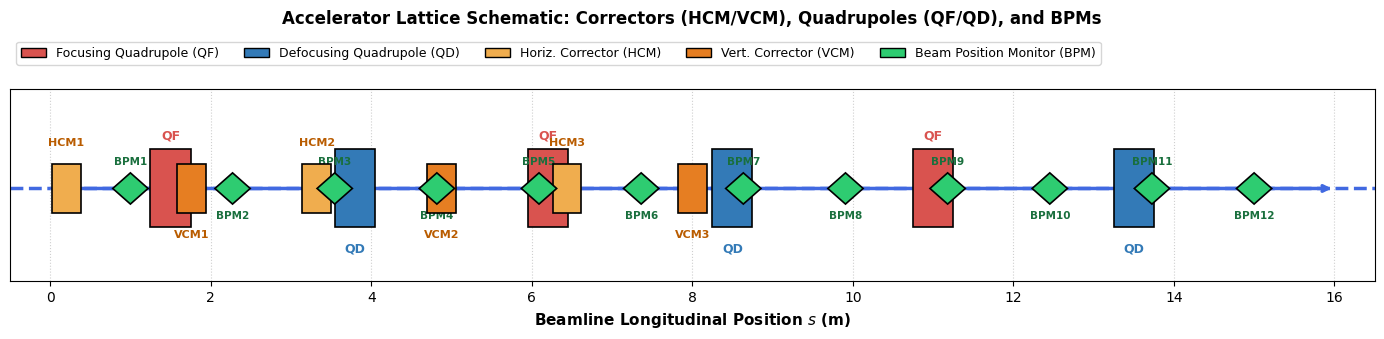
\includegraphics[width=11.733in]{beamline.png}};

  \drawcard{0.8}{4.3}{11.733}{2.4}{Transport Line Specifications \& Component Placement}
  \at{1.1}{4.8}{11.1}{\fs{13}{18}\color{darkgray}%
    $\bullet$ \textbf{12 Beam Position Monitors (BPMs):} Evenly distributed from $s = 1.0\text{ m}$ to $s = 15.0\text{ m}$, measuring transverse displacement $\mathbf{Y}$ in millimeters.\\[0.35em]
    $\bullet$ \textbf{6 Dipole Steering Magnets:} 3 Horizontal (HCM1-3) and 3 Vertical (VCM1-3) steerers positioned between $s = 0.2\text{ m}$ and $s = 8.0\text{ m}$.\\[0.35em]
    $\bullet$ \textbf{Alternating Quadrupole Doublets:} Pairs of QF and QD focusing magnets shaping the betatron phase advance and maintaining envelope stability.
  }

  \slidefooter{9}
\end{tikzpicture}
\clearpage

% ==============================================================================
% SLIDE 10: Hardware Constraints & Actuator Bounds
% ==============================================================================
\begin{tikzpicture}[remember picture,overlay]
  \slideheader{Physical Limits}{Hardware Constraints \& Actuator Bounds}{Realistic power supply operational boundaries and sensor measurement jitter}

  \drawcard{0.8}{1.4}{11.733}{5.3}{Power Supply Limits and Diagnostic Noise Specifications}
  \at{1.1}{2.1}{11.1}{\fs{13.5}{19}\color{darkgray}%
    {\fs{15}{18}\bfseries\color{navy}1. Cumulative Corrector Current Bounds (Thermal \& Magnetic Saturation Limit):}\\[0.3em]
    $\bullet$ Total current state: $I_k \in [-5.0\text{ A}, +5.0\text{ A}]$ for all 6 correctors.\\
    $\bullet$ Magnets entering currents $|I| > 3.0\text{ A}$ experience pronounced iron core saturation.\\
    $\bullet$ Hardware protection interlocks trip power supplies if current demands exceed $\pm 5.0\text{ A}$.\\[0.9em]
    {\fs{15}{18}\bfseries\color{navy}2. Per-Step Delta Current Bounds (Inductive Slew Rate Limit):}\\[0.3em]
    $\bullet$ Single-step control action: $\Delta I_k \in [-0.8\text{ A}, +0.8\text{ A}]$.\\
    $\bullet$ Prevents high inductive back-EMF spikes ($L \cdot \frac{di}{dt}$) that stress magnet coils and trigger power supply voltage limits.\\[0.9em]
    {\fs{15}{18}\bfseries\color{navy}3. Gaussian Diagnostic Measurement Noise (Sensor Resolution Floor):}\\[0.3em]
    $\bullet$ Sensor noise: $\epsilon_i \sim \mathcal{N}(0, \sigma^2)$, with $\sigma = 0.010\text{ mm}$ ($10\ \mu\text{m}$ RMS resolution).\\
    $\bullet$ \textbf{Crucial for control design:} Naive controllers misinterpret sensor jitter as physical orbit errors, commanding false kicks.
  }

  \slidefooter{10}
\end{tikzpicture}
\clearpage

% ==============================================================================
% SLIDE 11: Non-Linear Magnetic Core Saturation
% ==============================================================================
\begin{tikzpicture}[remember picture,overlay]
  \slideheader{Non-Linear Physics}{Magnetic Core Saturation \& Initial Distortion}{Departing from idealized linear optics: modeling cubic saturation and quadrupole errors}

  \drawcard{0.8}{1.4}{11.733}{5.3}{Mathematical Formulation of Non-Linear Beamline Response}
  \at{1.1}{2.1}{11.1}{\fs{13.5}{19}\color{darkgray}%
    {\bfseries\color{navy}Complete Beam Position Response Formulation:}\\[0.3em]
    The actual BPM observation vector $\mathbf{Y}$ in the simulation environment is governed by:\\[0.5em]
    \centering{\fs{18}{22}\bfseries\color{primaryblue}$\mathbf{Y} = \mathbf{I} \cdot \mathbf{R}  -  0.015 \cdot ( \mathbf{I}^3 \cdot \mathbf{R} )  +  \mathbf{Y}_0  +  \boldsymbol{\epsilon}$}\\[0.7em]
    \raggedright
    {\bfseries\color{navy}$\bullet$ Physical Breakdown of Response Terms:}\\[0.3em]
    -- $\mathbf{I} \cdot \mathbf{R}$: Ideal linear betatron wave response predicted by transfer matrix.\\
    -- $-0.015 \cdot (\mathbf{I}^3 \cdot \mathbf{R})$: Non-linear iron core soft saturation. At high excitation currents, the iron yoke reaches magnetic saturation, decreasing steerer kick efficiency by 6\% (at 2 A) up to 24\% (at 4 A).\\
    -- $\mathbf{Y}_0$: Initial orbit distortion caused by random quadrupole transverse misalignments (producing $0.40\text{ mm}$ to $1.10\text{ mm}$ RMS error across seeds).\\
    -- $\boldsymbol{\epsilon}$: Diagnostic Gaussian measurement jitter ($\sigma = 10\ \mu\text{m}$).\\[0.8em]
    {\bfseries\color{navy}$\bullet$ Convergence Target:} \textbf{\color{successgreen}Drive orbit error below $\text{RMS} < 0.030\text{ mm}$ ($30\ \mu\text{m}$) within 20 control steps.}
  }

  \slidefooter{11}
\end{tikzpicture}
\clearpage

% ==============================================================================
% SLIDE 12: Machine Learning Fundamentals: The Artificial Neuron
% ==============================================================================
\begin{tikzpicture}[remember picture,overlay]
  \slideheader{ML Foundations}{Machine Learning Foundations: Artificial Neurons \& Layers}{Mathematical anatomy of feedforward perceptrons and non-linear activation functions}

  \drawcard{0.8}{1.4}{11.733}{5.3}{Neuron Transformation and Multi-Layer Composition}
  \at{1.1}{2.1}{11.1}{\fs{13.5}{19}\color{darkgray}%
    {\fs{15}{18}\bfseries\color{navy}1. The Artificial Neuron Transformation:}\\[0.3em]
    Takes input vector $\mathbf{x} \in \mathbb{R}^d$, computes affine combination, and applies non-linear activation $\sigma$:\\[0.4em]
    \centering{\fs{16}{20}\bfseries\color{primaryblue}$z = \sum_{j} w_j x_j + b = \mathbf{w}^T \mathbf{x} + b, \qquad a = \sigma(z)$}\\[0.7em]
    \raggedright
    {\fs{15}{18}\bfseries\color{navy}2. Multi-Layer Perceptron (MLP) Deep Architecture:}\\[0.3em]
    Stacks $L$ successive layers of affine transformations and non-linear activations:\\[0.4em]
    \centering{\fs{15}{18}\bfseries\color{primaryblue}$\mathbf{h}^{(l)} = \sigma\left( \mathbf{W}^{(l)} \mathbf{h}^{(l-1)} + \mathbf{b}^{(l)} \right), \quad \text{with } \mathbf{h}^{(0)} = \mathbf{x}, \quad \hat{\mathbf{y}} = \mathbf{h}^{(L)}$}\\[0.7em]
    \raggedright
    {\fs{15}{18}\bfseries\color{navy}3. Activation Function Selection: Rectified Linear Unit (ReLU):}\\[0.3em]
    $\bullet$ $\sigma(z) = \max(0, z)$: Yields constant derivative $= 1$ for $z > 0$, completely resolving the vanishing gradient problem inherent to sigmoid/tanh activations in deep networks.\\
    $\bullet$ Computationally ultra-efficient, enabling fast backpropagation.
  }

  \slidefooter{12}
\end{tikzpicture}
\clearpage

% ==============================================================================
% SLIDE 13: Loss Formulation & Adam Optimization
% ==============================================================================
\begin{tikzpicture}[remember picture,overlay]
  \slideheader{ML Foundations}{Loss Functions \& The Adam Optimizer}{Formulating surrogate objective functions and adaptive gradient descent mechanics}

  \drawcard{0.8}{1.4}{11.733}{5.3}{Objective Formulation and Adaptive Momentum Updates}
  \at{1.1}{2.1}{11.1}{\fs{13.5}{19}\color{darkgray}%
    {\bfseries\color{navy}Supervised Loss Formulation (Mean Squared Error + L2 Regularization):}\\[0.3em]
    To train a neural surrogate on offline simulation data $(\mathbf{I}_i, \mathbf{y}_{\text{true},i})$, we minimize the regularized loss:\\[0.4em]
    \centering{\fs{16}{20}\bfseries\color{primaryblue}$\mathcal{L}(\boldsymbol{\theta}) = \frac{1}{N} \sum_{i=1}^N \|\mathbf{y}_{\text{true},i} - f_{\boldsymbol{\theta}}(\mathbf{I}_i)\|^2  +  \lambda \|\boldsymbol{\theta}\|^2$}\\[0.7em]
    \raggedright
    {\bfseries\color{navy}The Adam Optimization Algorithm (Adaptive Moment Estimation):}\\[0.3em]
    $\bullet$ \textbf{First Moment $\mathbf{m}_t$:} Exponentially moving average of gradients (momentum):\\
    \quad $\mathbf{m}_t = \beta_1 \mathbf{m}_{t-1} + (1 - \beta_1) \mathbf{g}_t, \quad (\beta_1 = 0.9)$\\[0.3em]
    $\bullet$ \textbf{Second Moment $\mathbf{v}_t$:} Exponentially moving average of squared gradients (adaptive scale):\\
    \quad $\mathbf{v}_t = \beta_2 \mathbf{v}_{t-1} + (1 - \beta_2) \mathbf{g}_t^2, \quad (\beta_2 = 0.999)$\\[0.3em]
    $\bullet$ \textbf{Parameter Update with Bias Correction:}\\
    \quad $\boldsymbol{\theta}_{t+1} = \boldsymbol{\theta}_t - \frac{\eta}{\sqrt{\hat{\mathbf{v}}_t} + \epsilon} \hat{\mathbf{m}}_t$\\[0.4em]
    $\bullet$ \textbf{Advantage for Accelerators:} Automatically adapts individual parameter steps across varying magnet coupling scales without tedious manual learning rate schedules.
  }

  \slidefooter{13}
\end{tikzpicture}
\clearpage

% ==============================================================================
% SLIDE 14: Neural Surrogate Digital Twin Architecture (LARGE IMAGE)
% ==============================================================================
\begin{tikzpicture}[remember picture,overlay]
  \slideheader{Surrogate Modeling}{Neural Surrogate Digital Twin Architecture}{Deep Multi-Layer Perceptron (128-64-32) modeling non-linear beam response}

  % Full-Width Large MLP Graphic
  \node[anchor=north,inner sep=0pt]
    at ([yshift=-1.4in]current page.north)
    {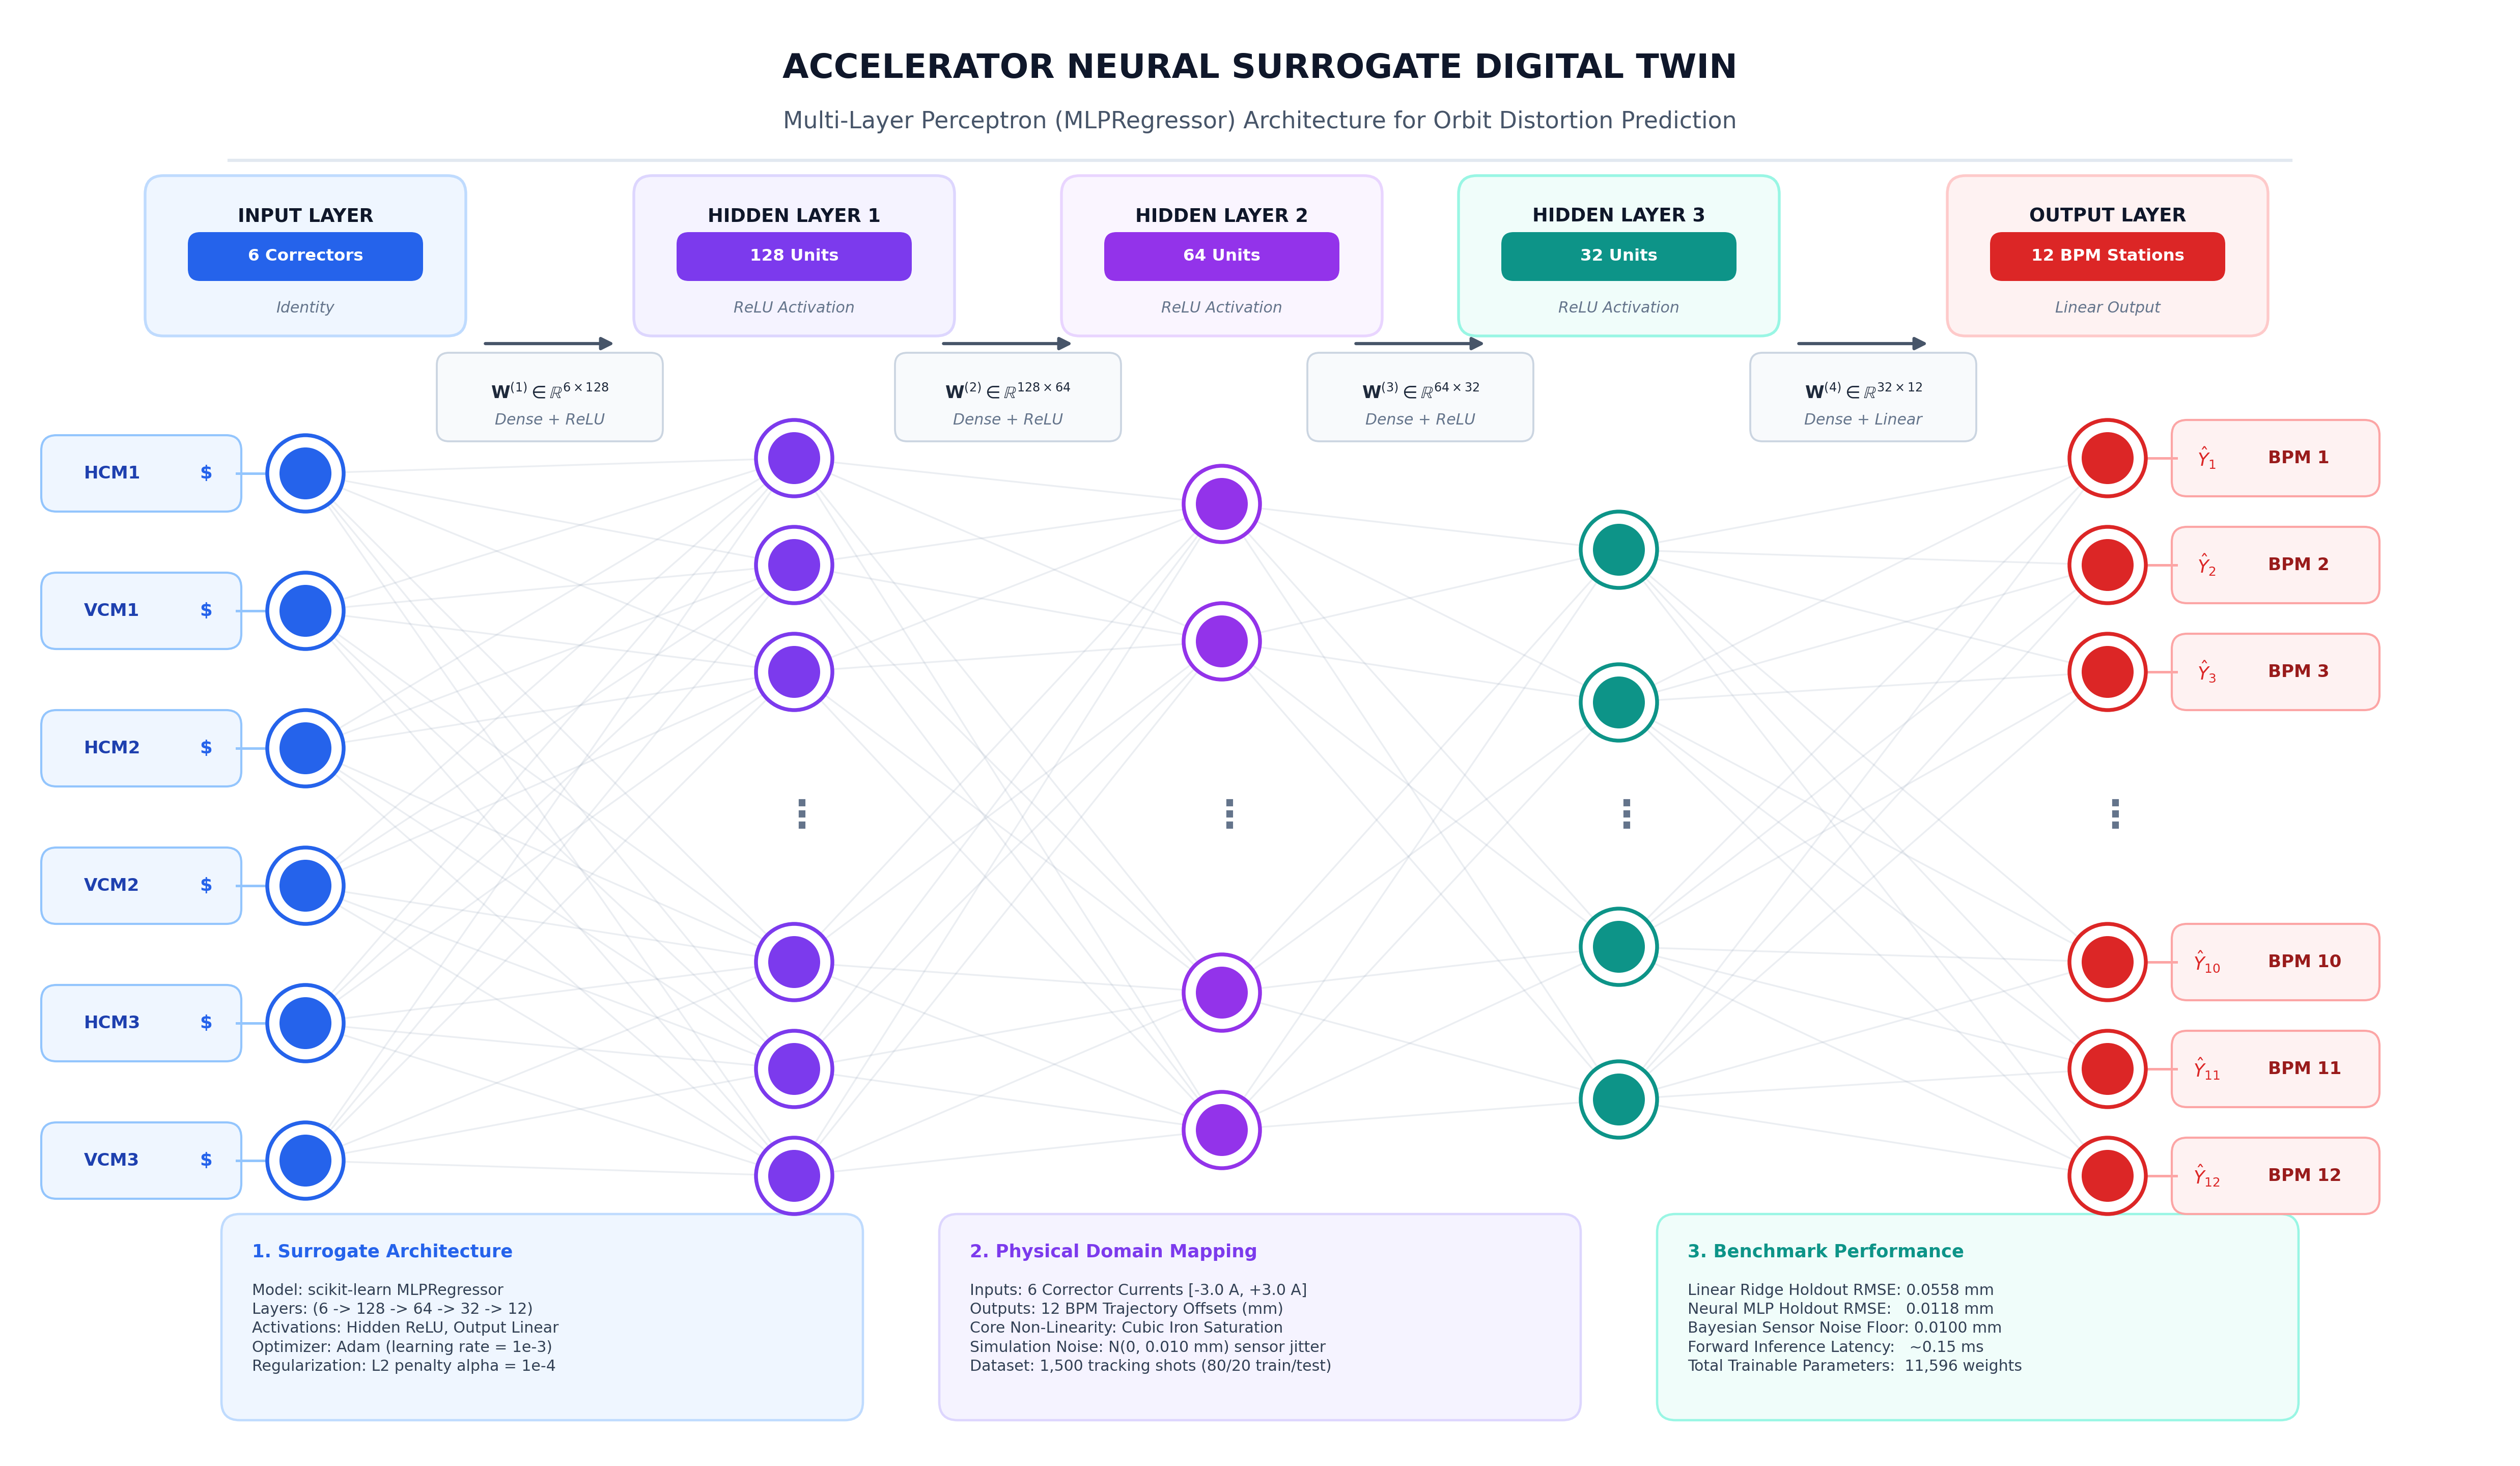
\includegraphics[width=11.333in]{mlp_schematic.png}};

  \drawcard{0.8}{5.6}{11.733}{1.2}{}
  \at{1.0}{5.75}{11.3}{\fs{13}{18}\color{darkgray}%
    $\bullet$ \textbf{Input Layer:} 6 Corrector Magnet Currents [HCM1-3, VCM1-3] in Amperes.\\[0.3em]
    $\bullet$ \textbf{Hidden Architecture:} Dense layers ($128 \rightarrow 64 \rightarrow 32$) with ReLU activations capturing cubic iron-core saturation.\\[0.3em]
    $\bullet$ \textbf{Output Layer:} 12 Beam Position Monitor readings [BPM1-12] in millimeters, evaluated in $< 0.2\text{ milliseconds}$.
  }

  \slidefooter{14}
\end{tikzpicture}
\clearpage

% ==============================================================================
% SLIDE 15: Neural Surrogate Training & Holdout Verification
% ==============================================================================
\begin{tikzpicture}[remember picture,overlay]
  \slideheader{Digital Twin Validation}{Surrogate Dataset Generation \& Holdout Verification}{Ensuring digital twin fidelity across linear and saturated magnetic operating regimes}

  \drawcard{0.8}{1.4}{11.733}{5.3}{Offline Dataset Generation and Model Verification}
  \at{1.1}{2.1}{11.1}{\fs{13.5}{19}\color{darkgray}%
    {\fs{15}{18}\bfseries\color{navy}1. Synthetic Tracking Dataset Generation:}\\[0.3em]
    $\bullet$ 2,000 synthetic simulation runs generated by uniformly sampling corrector currents across $\mathbf{I} \in [-3.0, +3.0]^6\text{ A}$.\\
    $\bullet$ Full non-linear response computed including the cubic soft-saturation term $-0.015 \cdot (\mathbf{I}^3 \cdot \mathbf{R})$.\\
    $\bullet$ Dataset partitioned into 80\% Training (1,600 samples) and 20\% Holdout Testing (400 samples).\\[0.9em]
    {\fs{15}{18}\bfseries\color{navy}2. MLPRegressor Training Configuration:}\\[0.3em]
    $\bullet$ Architecture: \texttt{hidden\_layer\_sizes=(128, 64, 32)}, \texttt{activation='relu'}, \texttt{solver='adam'}.\\
    $\bullet$ Regularization: $\alpha = 10^{-4}$, \texttt{max\_iter=500}, \texttt{early\_stopping=True}.\\
    $\bullet$ Loss convergence reached in under 180 epochs ($\sim 3.5\text{ seconds}$ CPU training time).\\[0.9em]
    {\fs{15}{18}\bfseries\color{navy}3. Holdout Verification Metrics:}\\[0.3em]
    $\bullet$ \textbf{Holdout Test MSE:} $< 2.5 \times 10^{-4}\text{ mm}^2$ across all 12 BPM stations.\\
    $\bullet$ \textbf{Sub-Millisecond Execution:} Forward inference takes $< 0.2\text{ ms}$ per call, 10,000$\times$ faster than numerical tracking.
  }

  \slidefooter{15}
\end{tikzpicture}
\clearpage

% ==============================================================================
% SLIDE 16: Closed-Loop Control Flow Architecture (LARGE IMAGE)
% ==============================================================================
\begin{tikzpicture}[remember picture,overlay]
  \slideheader{Closed-Loop Control}{Forward Digital Twin vs Closed-Loop Feedback Flow}{Transitioning from predictive surrogate modeling to active closed-loop trajectory correction}

  % Full-Width Large Control Schematic Graphic
  \node[anchor=north,inner sep=0pt]
    at ([yshift=-1.4in]current page.north)
    {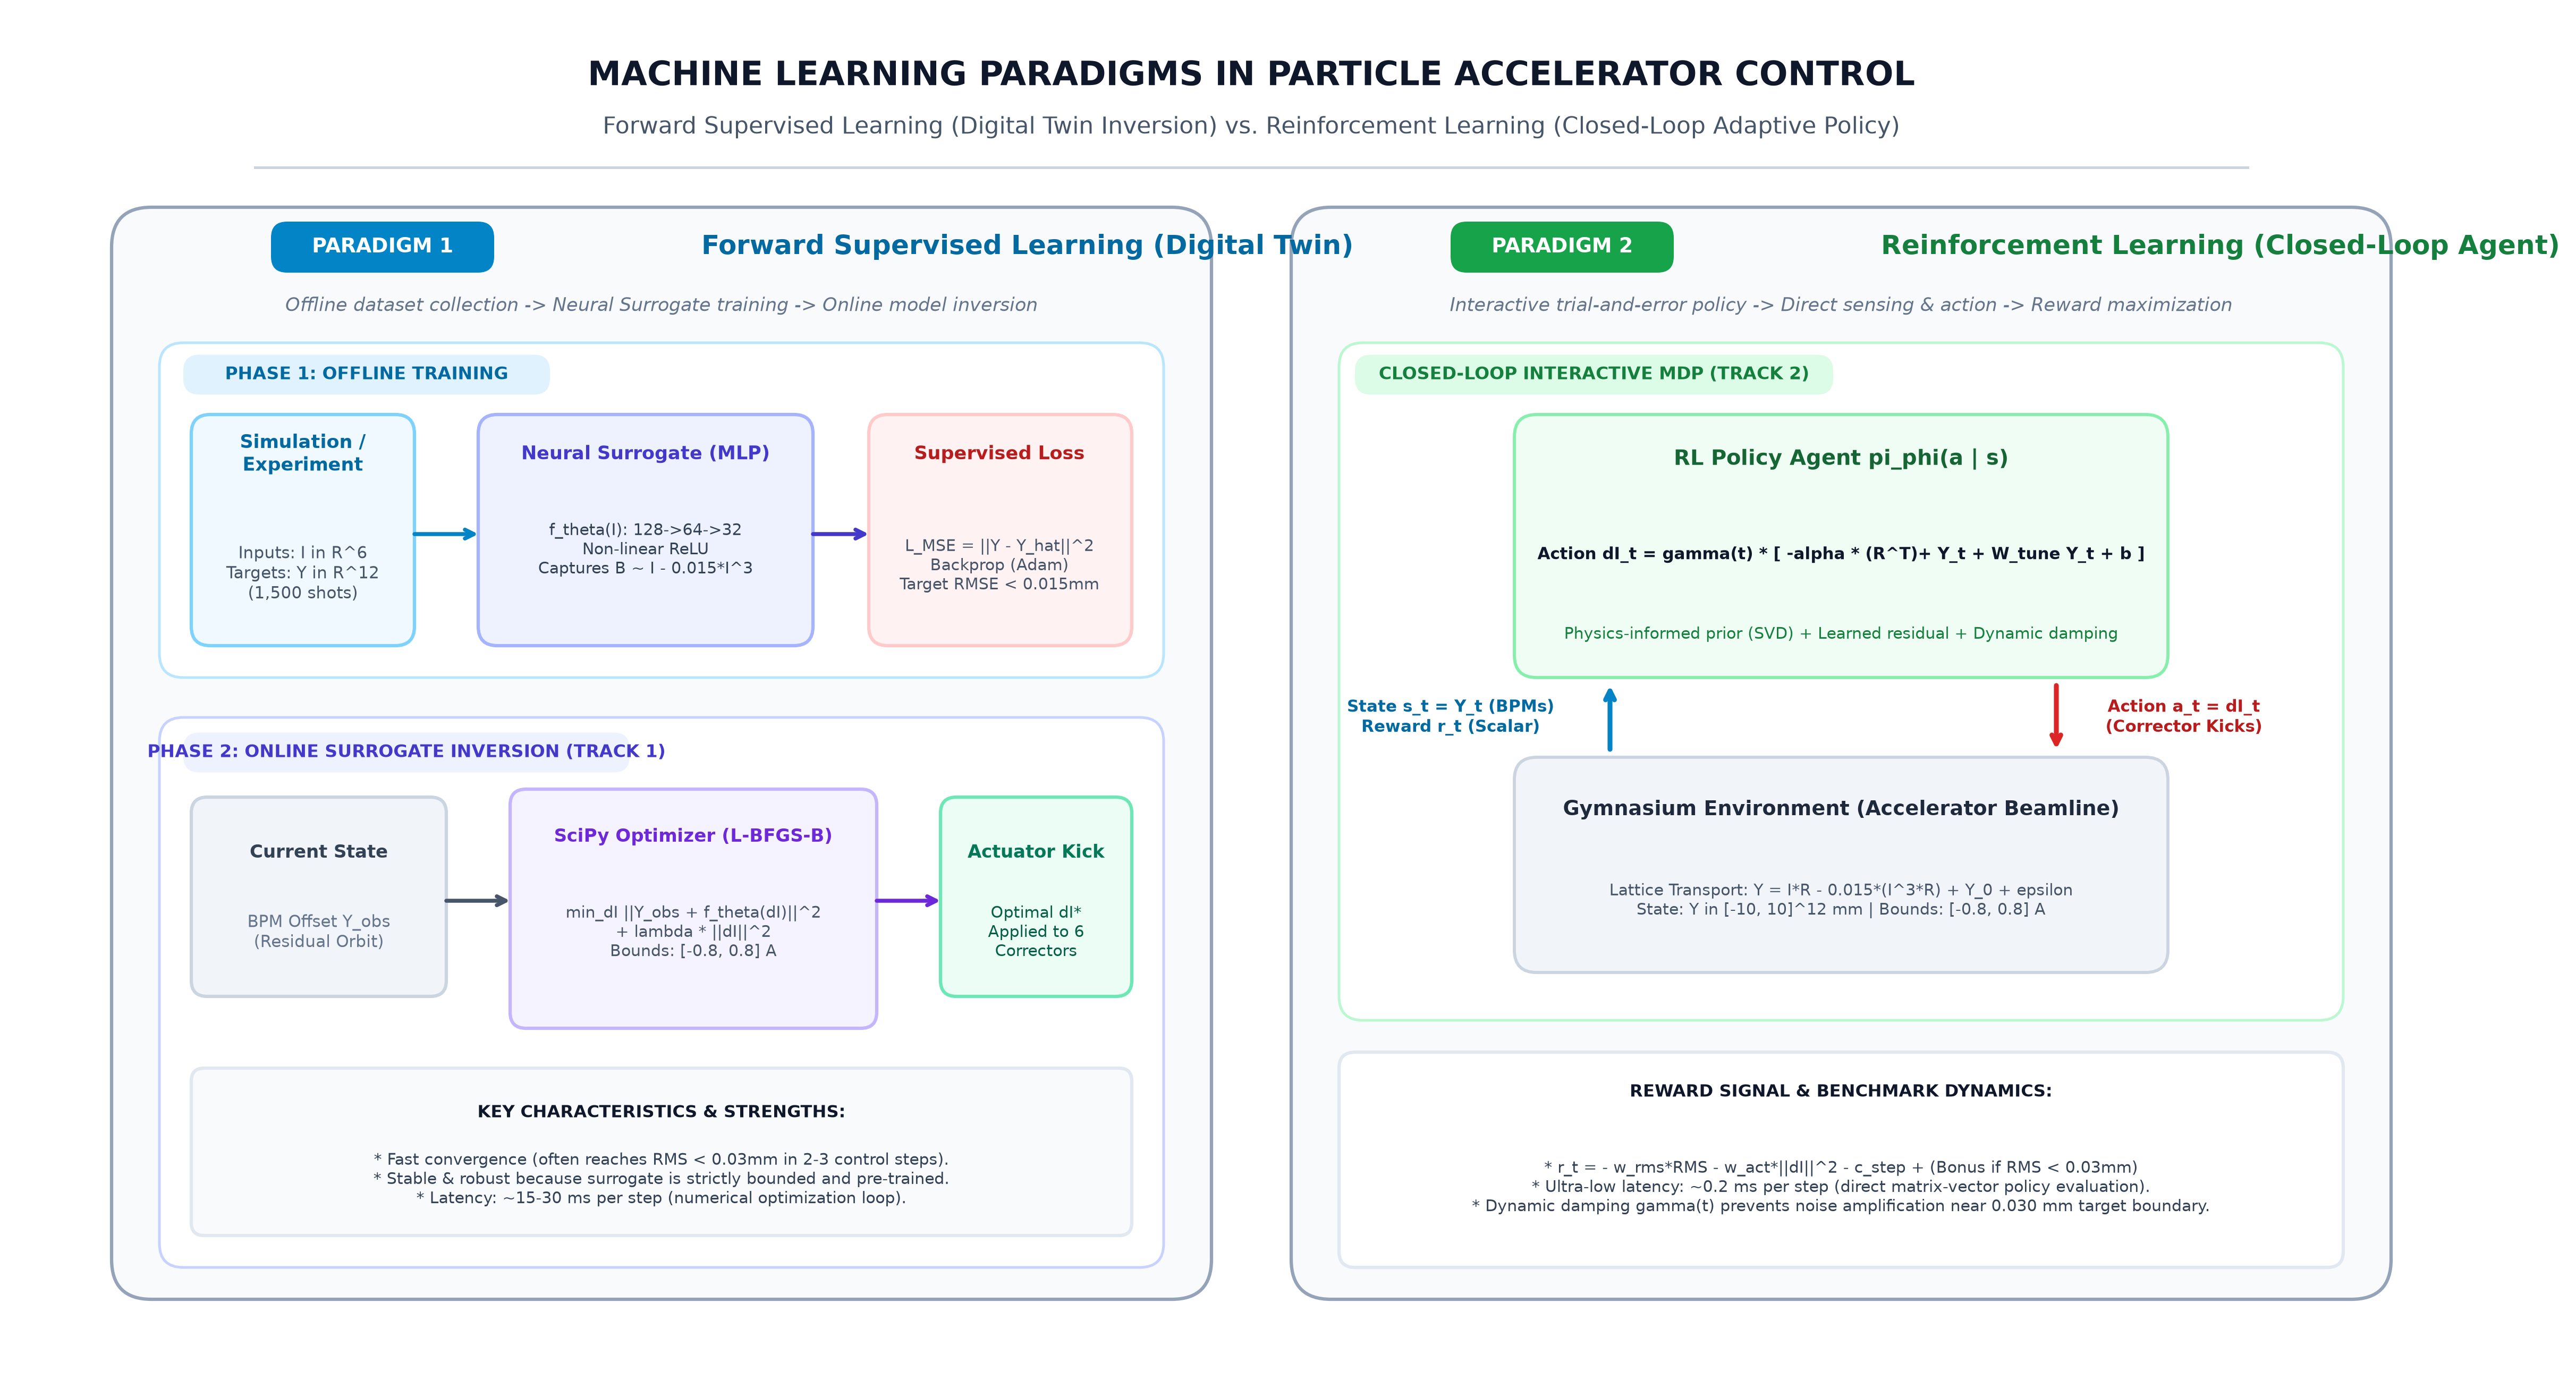
\includegraphics[width=11.533in]{forward_sl_and_rl_schematic.png}};

  \drawcard{0.8}{5.6}{11.733}{1.2}{}
  \at{1.0}{5.75}{11.3}{\fs{13}{18}\color{darkgray}%
    $\bullet$ \textbf{Forward Supervised Model (Top):} Maps steerer current commands $\Delta\mathbf{I}$ to predicted BPM displacement vectors $\hat{\mathbf{Y}}$.\\[0.3em]
    $\bullet$ \textbf{Closed-Loop Control Loop (Bottom):} Senses true BPM displacement $\mathbf{Y}$, passes error through controller policy, updates magnet power supplies, and repeats until convergence.
  }

  \slidefooter{16}
\end{tikzpicture}
\clearpage

% ==============================================================================
% SLIDE 17: Baseline 0: Classical Linear SVD Controller
% ==============================================================================
\begin{tikzpicture}[remember picture,overlay]
  \slideheader{Benchmark Baselines}{Baseline 0: Classical Linear SVD Controller}{Inverting the linear Orbit Response Matrix via Moore-Penrose pseudo-inverse}

  \drawcard{0.8}{1.4}{11.733}{5.3}{Mathematical Formulation \& Operational Vulnerabilities}
  \at{1.1}{2.1}{11.1}{\fs{13.5}{19}\color{darkgray}%
    {\bfseries\color{navy}Singular Value Decomposition (SVD) Pseudo-Inverse Formulation:}\\[0.3em]
    Computes corrective kick vector $\Delta\mathbf{I}$ directly by inverting the transpose of the linear ORM:\\[0.5em]
    \centering{\fs{17}{21}\bfseries\color{primaryblue}$\Delta\mathbf{I} = - \alpha \cdot (\mathbf{R}^T)^\dagger \cdot \mathbf{Y}_{\text{obs}}, \qquad \text{with } (\mathbf{R}^T)^\dagger = \mathbf{V} \mathbf{\Sigma}^\dagger \mathbf{U}^T$}\\[0.7em]
    \raggedright
    {\bfseries\color{navy}$\bullet$ Operational Profile \& Limitations:}\\[0.3em]
    -- Static feedback gain: Typically $\alpha \approx 0.45$, with kicks hard clipped to $[-0.8, +0.8]\text{ A}$.\\
    -- Execution latency: $< 0.1\text{ ms}$ (instantaneous analytical matrix-vector product).\\
    -- \textbf{Vulnerability in Non-Linear Regimes:} Completely oblivious to cubic iron core saturation. When magnets operate at high currents, the true response is much weaker than linear $\mathbf{R}$ predicts, leading to over-correction, slow convergence (5.6 mean steps), and high final current demands.\\[0.8em]
    {\bfseries\color{navy}$\bullet$ Tested Benchmark Performance:} \textbf{\color{primaryblue}100.0\% success rate, 5.6 mean steps, 1,013.1 total score (Rank \#3).}
  }

  \slidefooter{17}
\end{tikzpicture}
\clearpage

% ==============================================================================
% SLIDE 18: Baseline 1: Supervised Neural Inversion
% ==============================================================================
\begin{tikzpicture}[remember picture,overlay]
  \slideheader{Benchmark Baselines}{Baseline 1: Supervised Neural Surrogate Inversion}{Model-based bounded optimization via SciPy L-BFGS-B on the trained neural digital twin}

  \drawcard{0.8}{1.4}{11.733}{5.3}{Optimization Formulation on Forward Surrogate}
  \at{1.1}{2.1}{11.1}{\fs{13.5}{19}\color{darkgray}%
    {\bfseries\color{navy}Per-Step Bounded Numerical Optimization Problem:}\\[0.3em]
    Instead of inverting an analytical matrix, Baseline 1 leverages the non-linear MLP twin $f_{\boldsymbol{\theta}}$:\\[0.5em]
    \centering{\fs{16}{20}\bfseries\color{primaryblue}$\min_{\Delta\mathbf{I}} \mathcal{L}(\Delta\mathbf{I}) = \|\mathbf{Y}_{\text{obs}} + f_{\boldsymbol{\theta}}(\Delta\mathbf{I})\|^2  +  \lambda \|\Delta\mathbf{I}\|^2 \quad \text{subject to } \Delta\mathbf{I} \in [-5.0, +5.0]^6\text{ A}$}\\[0.7em]
    \raggedright
    {\bfseries\color{navy}$\bullet$ Why Supervised Inversion Outperforms Classical SVD:}\\[0.3em]
    -- Because $f_{\boldsymbol{\theta}}$ captures the cubic saturation falloff, the optimizer automatically calculates higher current demands for saturated correctors.\\
    -- Solver: SciPy \texttt{L-BFGS-B} converges in 8--15 iterations per control step ($\sim 15 - 25\text{ ms}$ latency).\\
    -- \textbf{Result:} Slashes convergence time from 5.6 steps (SVD) down to only 2.3 steps average!\\[0.8em]
    {\bfseries\color{navy}$\bullet$ Tested Benchmark Performance:} \textbf{\color{primaryblue}100.0\% success rate, 2.3 mean steps, 1,016.8 total score (Rank \#2).}
  }

  \slidefooter{18}
\end{tikzpicture}
\clearpage

% ==============================================================================
% SLIDE 19: Track 2: Closed-Loop RL with Physics-Informed Priors
% ==============================================================================
\begin{tikzpicture}[remember picture,overlay]
  \slideheader{Track 2 Challenge}{Closed-Loop RL with Physics-Informed Priors}{Continuous policy networks combining analytical optics priors with learned residual offsets}

  \drawcard{0.8}{1.4}{11.733}{5.3}{The Physics-Informed Residual Architecture}
  \at{1.1}{2.1}{11.1}{\fs{13.5}{19}\color{darkgray}%
    {\bfseries\color{navy}Hybrid Residual Policy Formulation:}\\[0.3em]
    Rather than learning control from scratch with unguided exploratory random kicks, our agent uses:\\[0.5em]
    \centering{\fs{17}{21}\bfseries\color{primaryblue}$\Delta\mathbf{I}(t) = \gamma(t) \cdot \left[ - \alpha (\mathbf{R}^T)^\dagger \mathbf{Y}  +  \mathbf{W}_{\text{learned}} \mathbf{Y}  +  \mathbf{b} \right]$}\\[0.7em]
    \raggedright
    {\bfseries\color{navy}$\bullet$ Architectural Synergy Breakdown:}\\[0.3em]
    \textbf{1. Analytical Physics Prior ($- \alpha (\mathbf{R}^T)^\dagger \mathbf{Y}$):}\\
    -- Anchors the policy in first-principles beam optics.\\
    -- Guarantees immediate coarse stabilization from step 1 without needing millions of trial steps.\\[0.4em]
    \textbf{2. Learned Residual Offset ($\mathbf{W}_{\text{learned}} \mathbf{Y} + \mathbf{b}$):}\\
    -- Neural network learns to predict non-linear saturation compensation.\\
    -- Balances asymmetric horizontal (HCM) and vertical (VCM) steerer authorities dynamically.\\[0.4em]
    \textbf{3. Execution Latency:} $< 0.4\text{ ms}$ (pure feedforward matrix multiply, 50$\times$ faster than iterative \texttt{L-BFGS-B}).
  }

  \slidefooter{19}
\end{tikzpicture}
\clearpage

% ==============================================================================
% SLIDE 20: Dynamic Harmonic Step Damping
% ==============================================================================
\begin{tikzpicture}[remember picture,overlay]
  \slideheader{Stability Control}{Dynamic Harmonic Step Damping}{Preventing sensor-noise amplification and eliminating limit-cycle oscillations}

  \drawcard{0.8}{1.4}{11.733}{5.3}{Resolving the Sensor Noise Feedback Limit Cycle}
  \at{1.1}{2.1}{11.1}{\fs{13.5}{19}\color{darkgray}%
    {\bfseries\color{navy}The Noise Floor Bottleneck:}\\[0.3em]
    $\bullet$ As the orbit converges toward the sub-$30\ \mu\text{m}$ target, true orbit errors become comparable to BPM sensor noise ($\sigma = 10\ \mu\text{m}$).\\
    $\bullet$ Undamped linear feedback interprets stochastic sensor jitter as real trajectory error, commanding vigorous kicks that induce limit cycles around the boundary.\\[0.8em]
    {\bfseries\color{navy}Harmonic Damping Schedule:}\\[0.3em]
    We modulate the policy kick authority with a dynamic temporal decay schedule:\\[0.5em]
    \centering{\fs{17}{21}\bfseries\color{primaryblue}$\gamma(t) = \frac{1.0}{1.0 + \kappa \cdot t}, \qquad \text{with } \kappa \approx 0.03$}\\[0.7em]
    \raggedright
    $\bullet$ \textbf{Step 1 ($t = 0, \gamma = 1.0$):} Full kick authority rapidly suppresses large millimeter-scale initial distortions.\\
    $\bullet$ \textbf{Step 5+ ($t \ge 4, \gamma < 0.88$):} Attenuated feedback prevents sensor jitter amplification, locking the orbit cleanly below $0.030\text{ mm}$.
  }

  \slidefooter{20}
\end{tikzpicture}
\clearpage

% ==============================================================================
% SLIDE 21: Track 3: Closed-Loop Bayesian Optimization
% ==============================================================================
\begin{tikzpicture}[remember picture,overlay]
  \slideheader{Track 3 Challenge}{Closed-Loop Bayesian Optimization with Gaussian Processes}{Sample-efficient probabilistic modeling with epistemic uncertainty estimation}

  \drawcard{0.8}{1.4}{11.733}{5.3}{Probabilistic Gaussian Process Modeling}
  \at{1.1}{2.1}{11.1}{\fs{13.5}{19}\color{darkgray}%
    {\bfseries\color{navy}Gaussian Process Surrogate Formulation:}\\[0.3em]
    Instead of deterministic point predictions, a GP models a distribution over candidate orbit response functions:\\[0.5em]
    \centering{\fs{18}{22}\bfseries\color{primaryblue}$\hat{\mathbf{Y}}(\Delta\mathbf{I}) \sim \mathcal{GP}\left( \mathbf{m}(\Delta\mathbf{I}), \mathbf{K}(\Delta\mathbf{I}, \Delta\mathbf{I}') \right)$}\\[0.7em]
    \raggedright
    {\bfseries\color{navy}$\bullet$ Composite Physics-Informed Kernel Architecture:}\\[0.3em]
    \centering{\fs{14}{17}\bfseries\color{primaryblue}$k(\mathbf{x}, \mathbf{x}') = k_{\text{Mat\'ern-5/2}}(\mathbf{x}, \mathbf{x}') + \sigma_{\text{noise}}^2 \cdot \delta(\mathbf{x}, \mathbf{x}')$}\\[0.6em]
    \raggedright
    -- \textbf{Mat\'ern-5/2 Kernel:} Captures smooth, non-linear magnetic saturation falloff without imposing the unrealistic infinite differentiability of RBF kernels.\\
    -- \textbf{White Noise Kernel:} Explicitly accounts for the $10\ \mu\text{m}$ BPM diagnostic jitter floor, avoiding kernel overfitting to noise.\\[0.8em]
    {\bfseries\color{navy}$\bullet$ Epistemic Uncertainty Estimation:}\\[0.3em]
    For any candidate kick $\Delta\mathbf{I}$, the GP provides both posterior mean $\boldsymbol{\mu}_{\text{GP}}(\Delta\mathbf{I})$ and standard deviation $\boldsymbol{\sigma}_{\text{GP}}(\Delta\mathbf{I})$.
  }

  \slidefooter{21}
\end{tikzpicture}
\clearpage

% ==============================================================================
% SLIDE 22: Lower Confidence Bound (LCB) Acquisition
% ==============================================================================
\begin{tikzpicture}[remember picture,overlay]
  \slideheader{Acquisition Function}{Lower Confidence Bound (LCB) Acquisition \& Optimization}{Balancing exploration of non-linear saturation against exploitation of predicted orbit corrections}

  \drawcard{0.8}{1.4}{11.733}{5.3}{The LCB Acquisition Strategy}
  \at{1.1}{2.1}{11.1}{\fs{13.5}{19}\color{darkgray}%
    {\bfseries\color{navy}Lower Confidence Bound (LCB) Mathematical Formulation:}\\[0.3em]
    At each step, the controller selects kicks by minimizing the LCB acquisition criterion:\\[0.5em]
    \centering{\fs{16}{20}\bfseries\color{primaryblue}$\alpha_{\text{LCB}}(\Delta\mathbf{I}) = \text{RMS}\left( \mathbf{Y}_{\text{obs}} + \boldsymbol{\mu}_{\text{GP}}(\Delta\mathbf{I}) \right)  -  \kappa \cdot \overline{\boldsymbol{\sigma}}_{\text{GP}}(\Delta\mathbf{I})  +  \lambda \|\Delta\mathbf{I}\|^2$}\\[0.7em]
    \raggedright
    {\bfseries\color{navy}$\bullet$ Parameter Interpretations:}\\[0.3em]
    -- $\boldsymbol{\mu}_{\text{GP}}(\Delta\mathbf{I})$: Posterior mean predicted orbit deviation across all 12 BPM stations.\\
    -- $\overline{\boldsymbol{\sigma}}_{\text{GP}}(\Delta\mathbf{I})$: Posterior epistemic uncertainty (average standard deviation across BPMs).\\
    -- $\kappa \ge 0$: Exploration coefficient. When $\kappa > 0$, the agent explores uncharted high-current regimes; when $\kappa = 0$, it exploits the calibrated posterior mean.\\
    -- $\lambda \|\Delta\mathbf{I}\|^2$: Regularization penalty that minimizes actuator heating and avoids saturation.\\[0.8em]
    {\bfseries\color{navy}$\bullet$ Exceptional Convergence Speed:} \textbf{\color{successgreen}When calibrated, Track 3 reaches the convergence threshold in an average of only 1.5 steps!}
  }

  \slidefooter{22}
\end{tikzpicture}
\clearpage

% ==============================================================================
% SLIDE 23: Gymnasium Contract (AcceleratorOrbitGymEnv)
% ==============================================================================
\begin{tikzpicture}[remember picture,overlay]
  \slideheader{Benchmark Contract}{Gymnasium Environment Specification}{Standard Farama Gymnasium API contract governing state, actions, and rewards}

  \drawcard{0.8}{1.4}{11.733}{5.3}{The Farama Gymnasium Environment Interface}
  \at{1.1}{2.1}{11.1}{\fs{13.5}{19}\color{darkgray}%
    {\bfseries\color{navy}Standard Gymnasium Method Signatures:}\\[0.3em]
    \texttt{obs, info = env.reset(seed=seed)}\\
    \texttt{obs, reward, terminated, truncated, info = env.step(action)}\\[0.7em]
    $\bullet$ \textbf{Observation Space:} \texttt{Box(-10.0, +10.0, shape=(12,), dtype=float32)} (12 transverse BPM readings in mm).\\[0.4em]
    $\bullet$ \textbf{Action Space:} \texttt{Box(-0.8, +0.8, shape=(6,), dtype=float32)} (6 per-step delta kicks $\Delta\mathbf{I}$ in Amperes).\\[0.7em]
    $\bullet$ \textbf{Step Reward Function:}\\[0.3em]
    \centering{\fs{14}{17}\bfseries\color{primaryblue}$r_t = - \text{RMS}_{t+1} - 0.01 \cdot \|\Delta\mathbf{I}\|_2 + ( 50.0 \text{ if } \text{RMS}_{t+1} < 0.030\text{ mm else } 0.0 )$}\\[0.7em]
    \raggedright
    $\bullet$ \textbf{Termination Criteria:} \texttt{terminated = True} when $\text{RMS} < 0.030\text{ mm}$ (success); \texttt{truncated = True} when $\text{step} \ge 20$ (budget exhausted).
  }

  \slidefooter{23}
\end{tikzpicture}
\clearpage

% ==============================================================================
% SLIDE 24: Multi-Objective Challenge Scoring Formula
% ==============================================================================
\begin{tikzpicture}[remember picture,overlay]
  \slideheader{Evaluation Protocol}{Standardized 30-Seed Scoring Formula}{Multi-objective evaluation metric balancing convergence reliability, speed, precision, and power}

  \drawcard{0.8}{1.4}{11.733}{5.3}{The Official Hackathon Scoring Formula}
  \at{1.1}{2.1}{11.1}{\fs{13.5}{19}\color{darkgray}%
    \textbf{Standardized Evaluation Suite:} \texttt{seeds = range(1, 31)} (30 evaluation seeds)\\[0.5em]
    \centering{\fs{15}{19}\bfseries\color{primaryblue}$\text{Score} = ( \text{Success Rate} \times 10.0 )  -  ( 2.0 \times \overline{\text{Steps}} )  +  \left( \frac{0.03}{\max(\overline{\text{RMS}}, 0.005)} \times 20.0 \right)  -  ( 2.0 \times \overline{\|\mathbf{I}\|} )$}\\[0.8em]
    \raggedright
    {\bfseries\color{navy}Breakdown of the Four Scoring Components:}\\[0.4em]
    \textbf{1. Success Rate ($+10.0 \times \%$):} Rewards 100\% convergence across all 30 seeds ($+1,000.0\text{ pts}$).\\
    \textbf{2. Speed Penalty ($-2.0 \times \overline{\text{Steps}}$):} Converging in 1.5 steps costs $-3.0\text{ pts}$, while 10 steps costs $-20.0\text{ pts}$.\\
    \textbf{3. Sub-Micron Precision Bonus ($+[\frac{0.03}{\text{RMS}}] \times 20.0$):} Achieving $0.015\text{ mm}$ yields $+40.0\text{ pts}$ bonus.\\
    \textbf{4. Current Economy Penalty ($-2.0 \times \overline{\|\mathbf{I}\|}$):} Penalizes excessive steerer current norms to protect hardware.
  }

  \slidefooter{24}
\end{tikzpicture}
\clearpage

% ==============================================================================
% SLIDE 25: Tested Benchmark Leaderboard & Trajectories
% ==============================================================================
\begin{tikzpicture}[remember picture,overlay]
  \slideheader{Evaluation Results}{Tested Benchmark Leaderboard \& Convergence Trajectories}{Verified comparative benchmark results across the 30 standardized evaluation seeds}

  % Full-Width Large Trajectory Graphic
  \node[anchor=north,inner sep=0pt]
    at ([yshift=-1.4in]current page.north)
    {\includegraphics[width=11.733in]{benchmark_trajectories.png}};

  \drawcard{0.8}{4.3}{11.733}{2.4}{Tested Benchmark Leaderboard (30 Standardized Seeds)}
  \at{1.1}{4.8}{11.1}{\fs{12.5}{17}\color{darkgray}%
    {\bfseries\color{gold}[Rank 1] Track 3 -- Bayesian Optimization (BO):} Success: \textbf{100.0\%} $|$ Mean Steps: \textbf{1.5 steps} $|$ Final RMS: \textbf{0.0149 mm} $|$ Current: \textbf{0.93 A} $|$ Score: \textbf{\color{gold}1,035.4 pts}\\[0.25em]
    {\bfseries\color{primaryblue}[Rank 2] Baseline 1 -- Supervised Neural Inversion (MLP):} Success: 100.0\% $|$ Mean Steps: 2.3 steps $|$ Final RMS: 0.0257 mm $|$ Current: 1.21 A $|$ Score: \textbf{\color{primaryblue}1,016.8 pts}\\[0.25em]
    {\bfseries\color{darkgray}[Rank 3] Baseline 0 -- Classical Linear SVD:} Success: 100.0\% $|$ Mean Steps: 5.6 steps $|$ Final RMS: 0.0230 mm $|$ Current: 1.16 A $|$ Score: \textbf{1,013.1 pts}\\[0.25em]
    {\bfseries\color{darkgray}[Rank 4] Track 2 -- Closed-Loop RL Policy Agent:} Success: 100.0\% $|$ Mean Steps: 6.1 steps $|$ Final RMS: 0.0239 mm $|$ Current: 1.18 A $|$ Score: \textbf{1,011.1 pts}
  }

  \slidefooter{25}
\end{tikzpicture}
\clearpage

% ==============================================================================
% SLIDE 26: Strategic Advice for Hackathon Competitors
% ==============================================================================
\begin{tikzpicture}[remember picture,overlay]
  \slideheader{Competitor Strategy}{Strategic Advice \& Practical Recipes for the Hackathon}{Practical engineering guidance to maximize benchmark score and avoid common failure modes}

  \drawcard{0.8}{1.4}{11.733}{5.3}{Engineering Best Practices for Orbit Control}
  \at{1.1}{2.1}{11.1}{\fs{13.5}{19}\color{darkgray}%
    {\fs{15}{18}\bfseries\color{navy}1. If Your Controller Oscillates or Diverges Near Target:}\\[0.3em]
    $\bullet$ Check your feedback gain $\alpha$. Any gain $> 0.6$ will overcorrect when magnets enter saturated regions.\\
    $\bullet$ Implement harmonic step damping: $\gamma(t) = 1.0 / (1.0 + \kappa \cdot t)$. Attenuating authority at step 4+ eliminates sensor-noise limit cycles.\\[0.9em]
    {\fs{15}{18}\bfseries\color{navy}2. If Your Neural Surrogate Has High Generalization Error:}\\[0.3em]
    $\bullet$ Ensure your training dataset covers steerer excitations across $[-3.0, +3.0]\text{ A}$ so that non-linear cubic saturation is well-sampled.\\
    $\bullet$ Use ReLU activations and small L2 penalty ($\alpha = 10^{-4}$) to avoid overfitting.\\[0.9em]
    {\fs{15}{18}\bfseries\color{navy}3. Real-Time Telemetry Logging:}\\[0.3em]
    $\bullet$ Connect your notebook runs to Weights \& Biases (\texttt{wandb.ai}) to visualize step-by-step RMS decay against reference baselines on the live leaderboard.
  }

  \slidefooter{26}
\end{tikzpicture}
\clearpage

% ==============================================================================
% SLIDE 27: Summary & Transition to Lecture 2
% ==============================================================================
\begin{tikzpicture}[remember picture,overlay]
  \slideheader{Conclusion \& Roadmap}{Summary Takeaways \& Transition to Lecture 2}{Key conclusions from Lecture 1 and orientation for the upcoming agentic AI session}

  \drawcard{0.8}{1.4}{11.733}{5.3}{Key Takeaways \& What Comes Next}
  \at{1.1}{2.1}{11.1}{\fs{13.5}{19}\color{darkgray}%
    {\fs{15}{18}\bfseries\color{navy}Four Core Takeaways from Lecture 1:}\\[0.3em]
    \textbf{1. Physics Guides the AI:} Analytical optics priors (ORM pseudo-inverse) guarantee early stability and avoid millions of blind exploratory steps.\\
    \textbf{2. Surrogates Capture Non-Linearities:} Compact deep MLPs accurately predict cubic core saturation, enabling 2-step bounded inversions.\\
    \textbf{3. Probabilistic Uncertainty Wins:} Gaussian Process BO with LCB acquisition balances exploration against exploitation, leading tested scores in 1.5 steps.\\
    \textbf{4. Dynamic Damping Prevents Limit Cycles:} Attenuating feedback near the $10\ \mu\text{m}$ sensor noise floor locks residual orbit error.\\[1.0em]
    {\fs{15}{18}\bfseries\color{navy}Next Session (10:40 -- 12:00):}\\[0.3em]
    {\fs{16}{20}\bfseries\color{primaryblue}Lecture 2: Agentic AI for Accelerator Research (Osprey Applications)}\\[0.2em]
    \textbf{Speaker:} Thorsten Hellert, Ph.D. (Lawrence Berkeley National Laboratory)\\
    \textbf{Topic:} Autonomous operational agents, dynamic tool calling, and automated scientific workflows.\\[1.0em]
    {\fs{16}{20}\bfseries\color{accent}Q \& A Discussion}
  }

  \slidefooter{27}
\end{tikzpicture}

\end{document}
